\def\widerfacefourk{
    Kế thừa những điểm mạnh về sự đa dạng của khuôn mặt trong bộ dữ liệu WIDER FACE \cite{yang2016wider}, tôi đề xuất một phương pháp xây dựng bộ dữ liệu WIDER FACE 4K gồm có nhiều ảnh có kích thước lớn, giúp đánh giá khách quan độ chính xác và tốc độ của các mô hình giải bài toán nhận diện khuôn mặt với ảnh chất lượng cao.

    \subsubsection*{Ý tưởng xây dựng bộ dữ liệu WIDER FACE 4K}
    Nhằm tận dụng hết những điểm mạnh như tỷ lệ kích thước, kiểu dáng, biểu cảm, che chắn, góc quay và ánh sáng của bộ dữ liệu WIDER FACE, tôi không tác động gì đến dữ liệu ảnh của bộ dữ liệu WIDER FACE mà chỉ nối chúng lại với nhau theo dạng lưới nhằm tạo ra bộ dữ liệu ảnh có kích thước lớn hơn.
    Với số lượng cũng như độ đa dạng của khuôn mặt được giữ nguyên của bộ dữ liệu WIDER FACE, nhưng với kích thước ảnh lớn hơn, bộ dữ liệu WIDER FACE 4K sẽ đánh giá tốt khả năng của các mô hình nhận diện khuôn mặt, không chỉ ở độ chính xác, mà còn ở thời gian chạy cũng như khối lượng bộ nhớ cần dùng.

    \noindent
    Trong khuôn khổ của luận văn, tôi chỉ xây dựng các bộ dữ liệu WIDER FACE 4K với dạng lưới có kích thước $2 \times 2$, $3 \times 3$, $4 \times 4$ và $5 \times 5$, tuy nhiên, ý tưởng xây dựng bộ dữ liệu WIDER FACE 4K này hoàn toàn có thể áp dụng với các kích thước lưới lớn hơn $n \times n$ nhằm tạo ra bộ dữ liệu ảnh có kích thước lớn hơn nữa.

    \subsubsection*{Các thông số của bộ dữ liệu WIDER FACE 4K}
    Bộ dữ liệu WIDER FACE 4K, đúng với mục đích ra đời, đã làm tăng kích thước dữ liệu ảnh đáng kể.
    So sánh với bộ dữ liệu WIDER FACE với kích thước ảnh trung bình nằm trong khoảng từ 750 đến 1250 điểm ảnh mỗi chiều, bộ dữ liệu WIDER FACE 4K đã tăng kích thước ảnh trung bình từ 1500 đến 2500 điểm ảnh mỗi chiều đối với dạng lưới $2 \times 2$, 2200 đến 4000 điểm ảnh mỗi chiều đối với dạng lưới $3 \times 3$, 3000 đến 5000 điểm ảnh mỗi chiều đối với dạng lưới $4 \times 4$ và 4000 đến 6000 điểm ảnh mỗi chiều đối với dạng lưới $5 \times 5$.

    \begin{figure}[H]
        \centering
        \subfigure[]{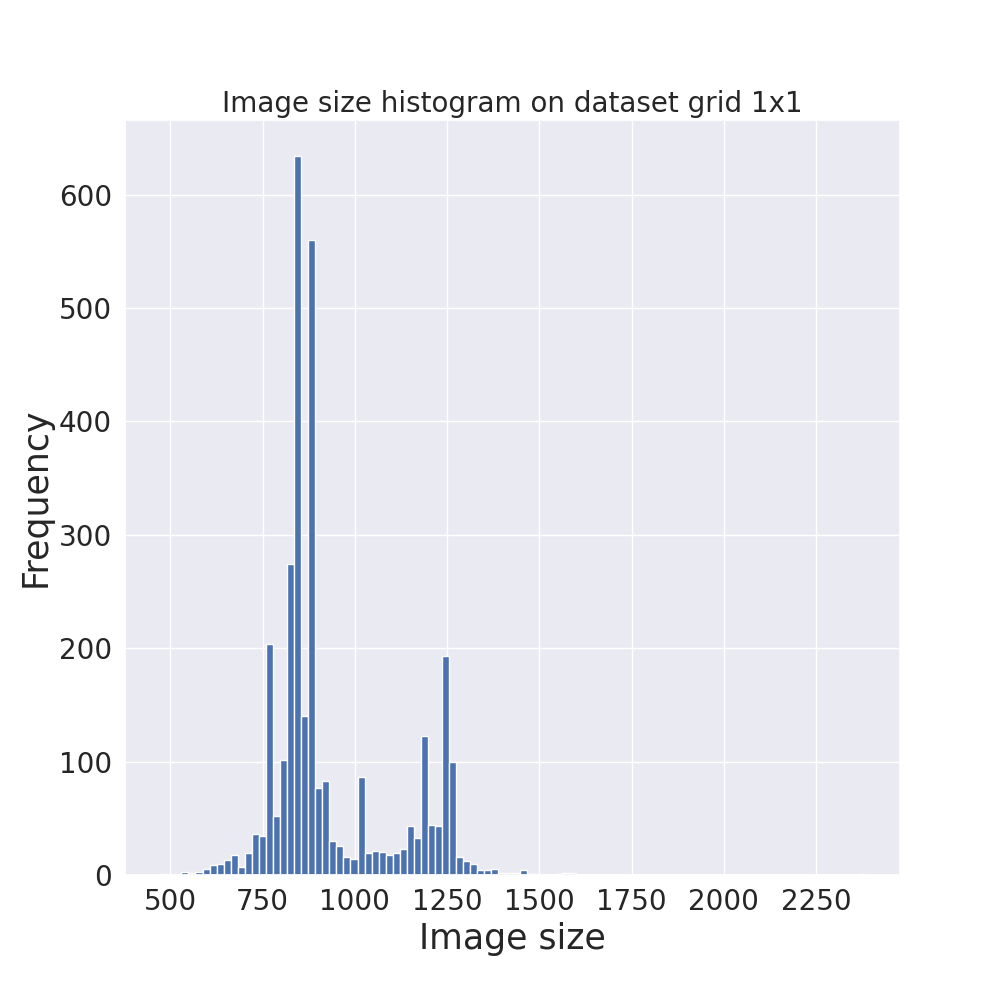
\includegraphics[width=5.5cm]{images/widerface_nk_img_size_1K}}
        \subfigure[]{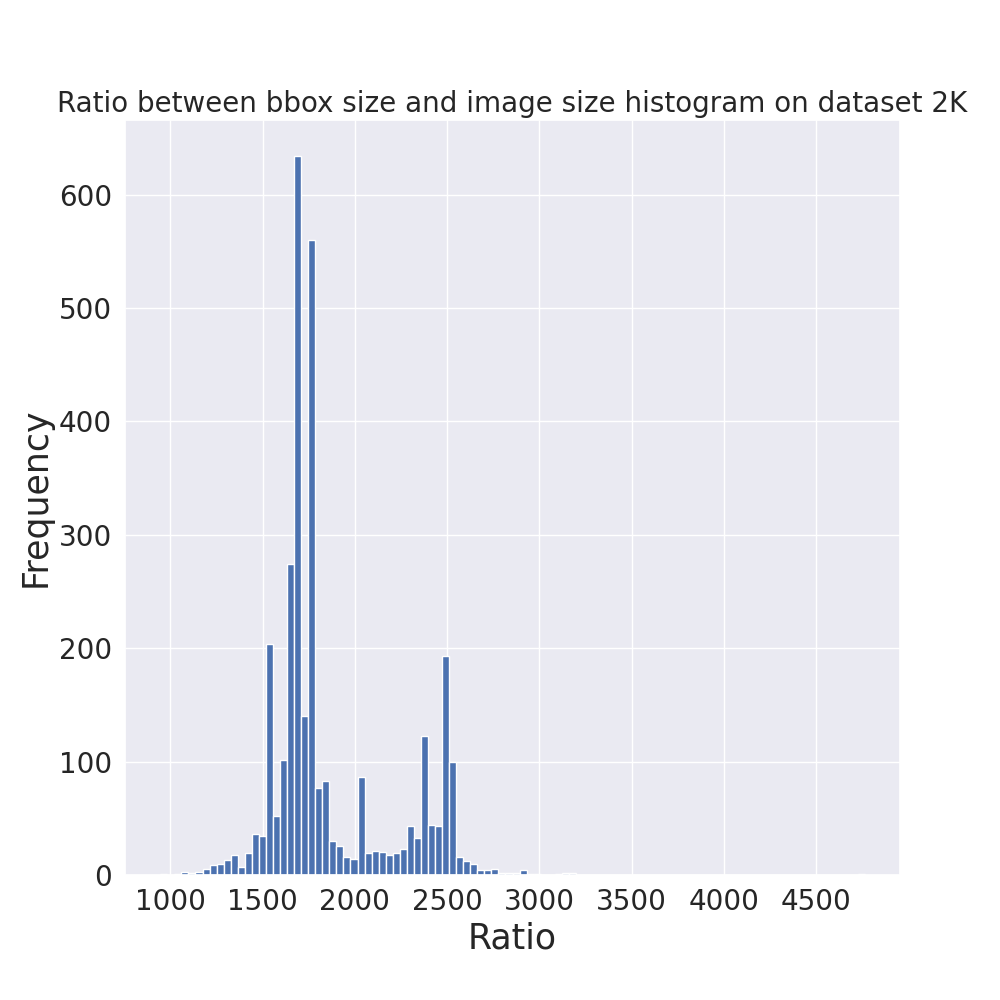
\includegraphics[width=5.5cm]{images/widerface_nk_img_size_2K}}
        \subfigure[]{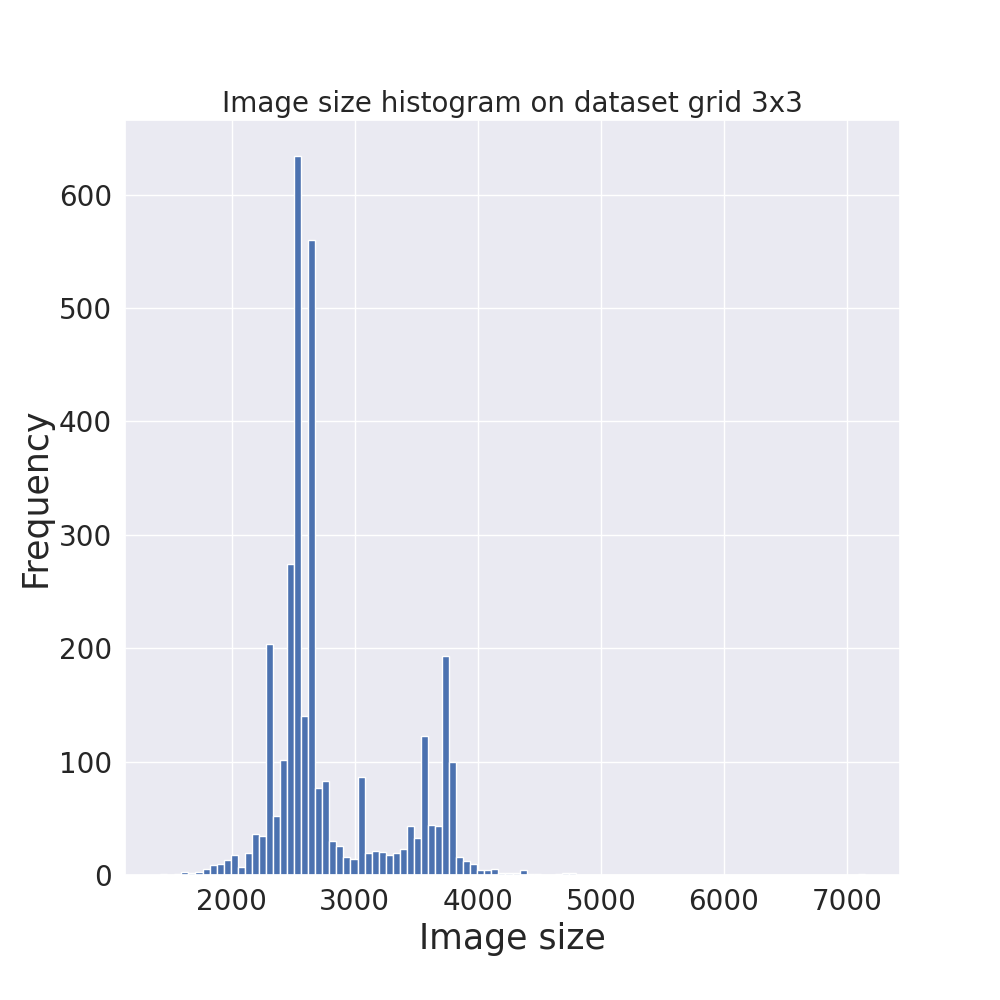
\includegraphics[width=5.5cm]{images/widerface_nk_img_size_3K}}
        \subfigure[]{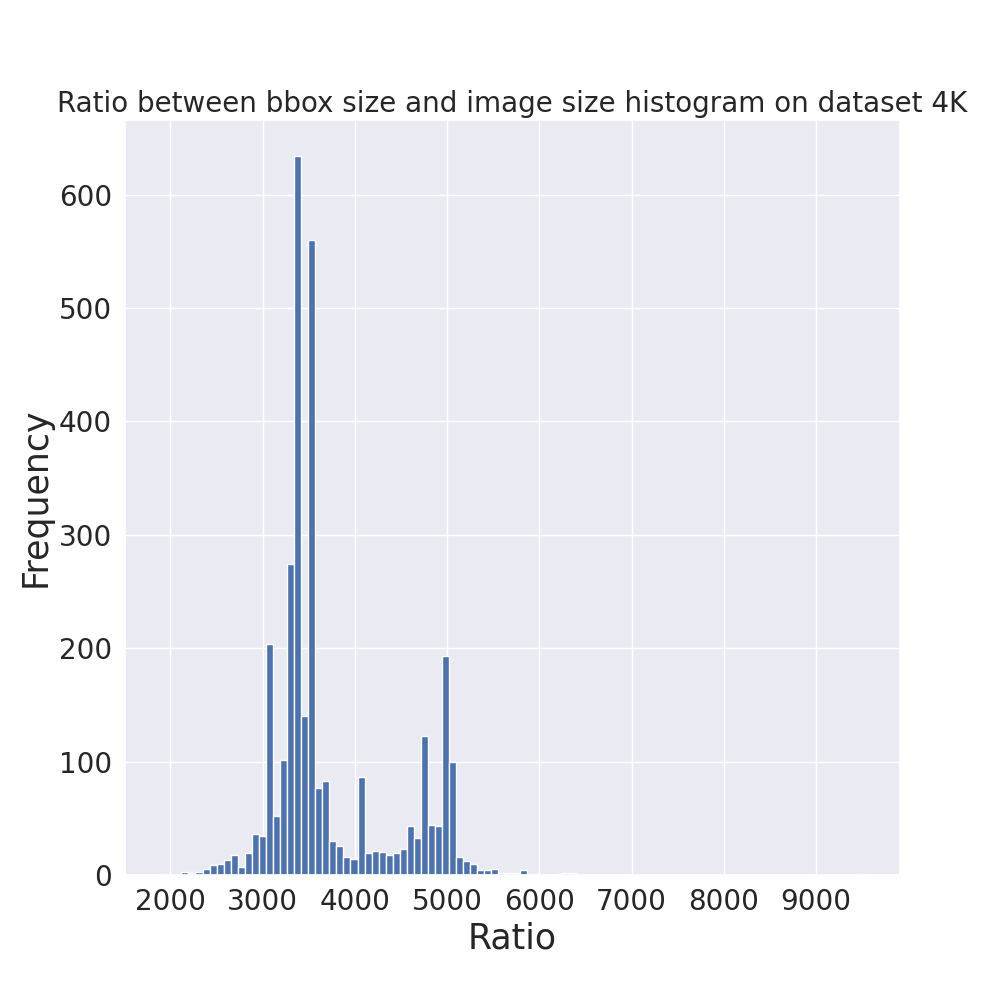
\includegraphics[width=5.5cm]{images/widerface_nk_img_size_4K}}
        \subfigure[]{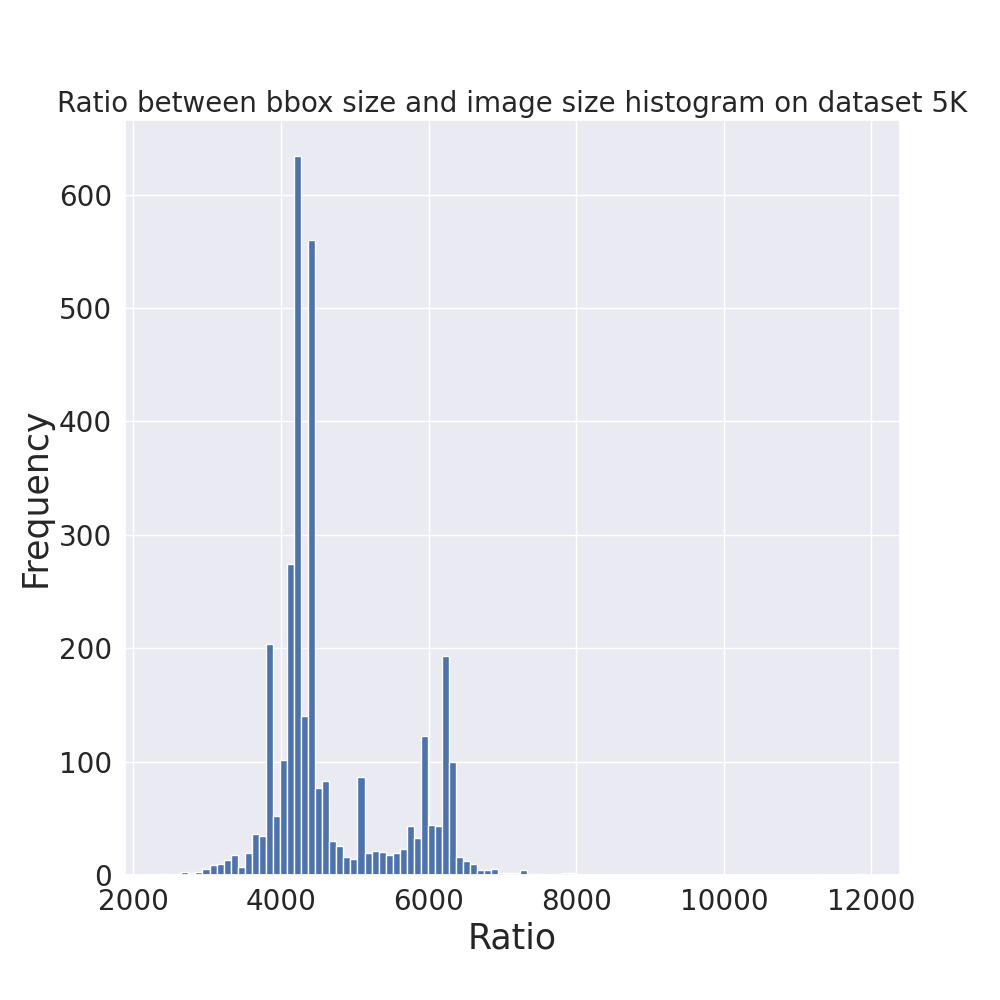
\includegraphics[width=5.5cm]{images/widerface_nk_img_size_5K}}
        \caption{Phân phối về kích thước ảnh trong bộ dữ liệu WIDER FACE \cite{yang2016wider} (a) so sánh với bộ dữ liệu WIDER FACE 4K dạng lưới $2 \times 2$ (b), $3 \times 3$ (c), $4 \times 4$ (d) và $5 \times 5$ (d)}
        \label{fig:widerface_4k_img_size}
    \end{figure}

    \noindent
    Hơn nữa, kích thước ảnh tối đa trên bộ dữ liệu WIDER FACE 4K cũng được cải thiện, so sánh với kích thước 2250 điểm ảnh của bộ dữ liệu WIDER FACE, bộ dữ liệu WIDER FACE 4K có kích thước ảnh tối đa là 4500 điểm ảnh với dạng lưới $2 \times 2$, 7000 điểm ảnh với dạng lưới $3 \times 3$, 9000 điểm ảnh với dạng lưới $4 \times 4$ và 12000 điểm ảnh với dạng lưới $5 \times 5$.

    \noindent
    Với việc kích thước ảnh được tăng lên đáng kể, việc nhận diện các khuôn mặt trong ảnh trở nên khó khăn hơn, đặc biệt là với các khuôn mặt có kích thước nhỏ.
    Trong bộ dữ liệu WIDER FACE 4K, số lượng các mặt có kích thước nhỏ so sánh tỷ lệ với kích thước ảnh trong bộ dữ liệu lớn hơn.
    Cụ thể, đối với bộ dữ liệu WIDER FACE, trung bình kích thước hộp giới hạn của khuôn mặt bằng khoảng 2\% kích thước của ảnh.

    \begin{figure}[H]
        \centering
        \subfigure[]{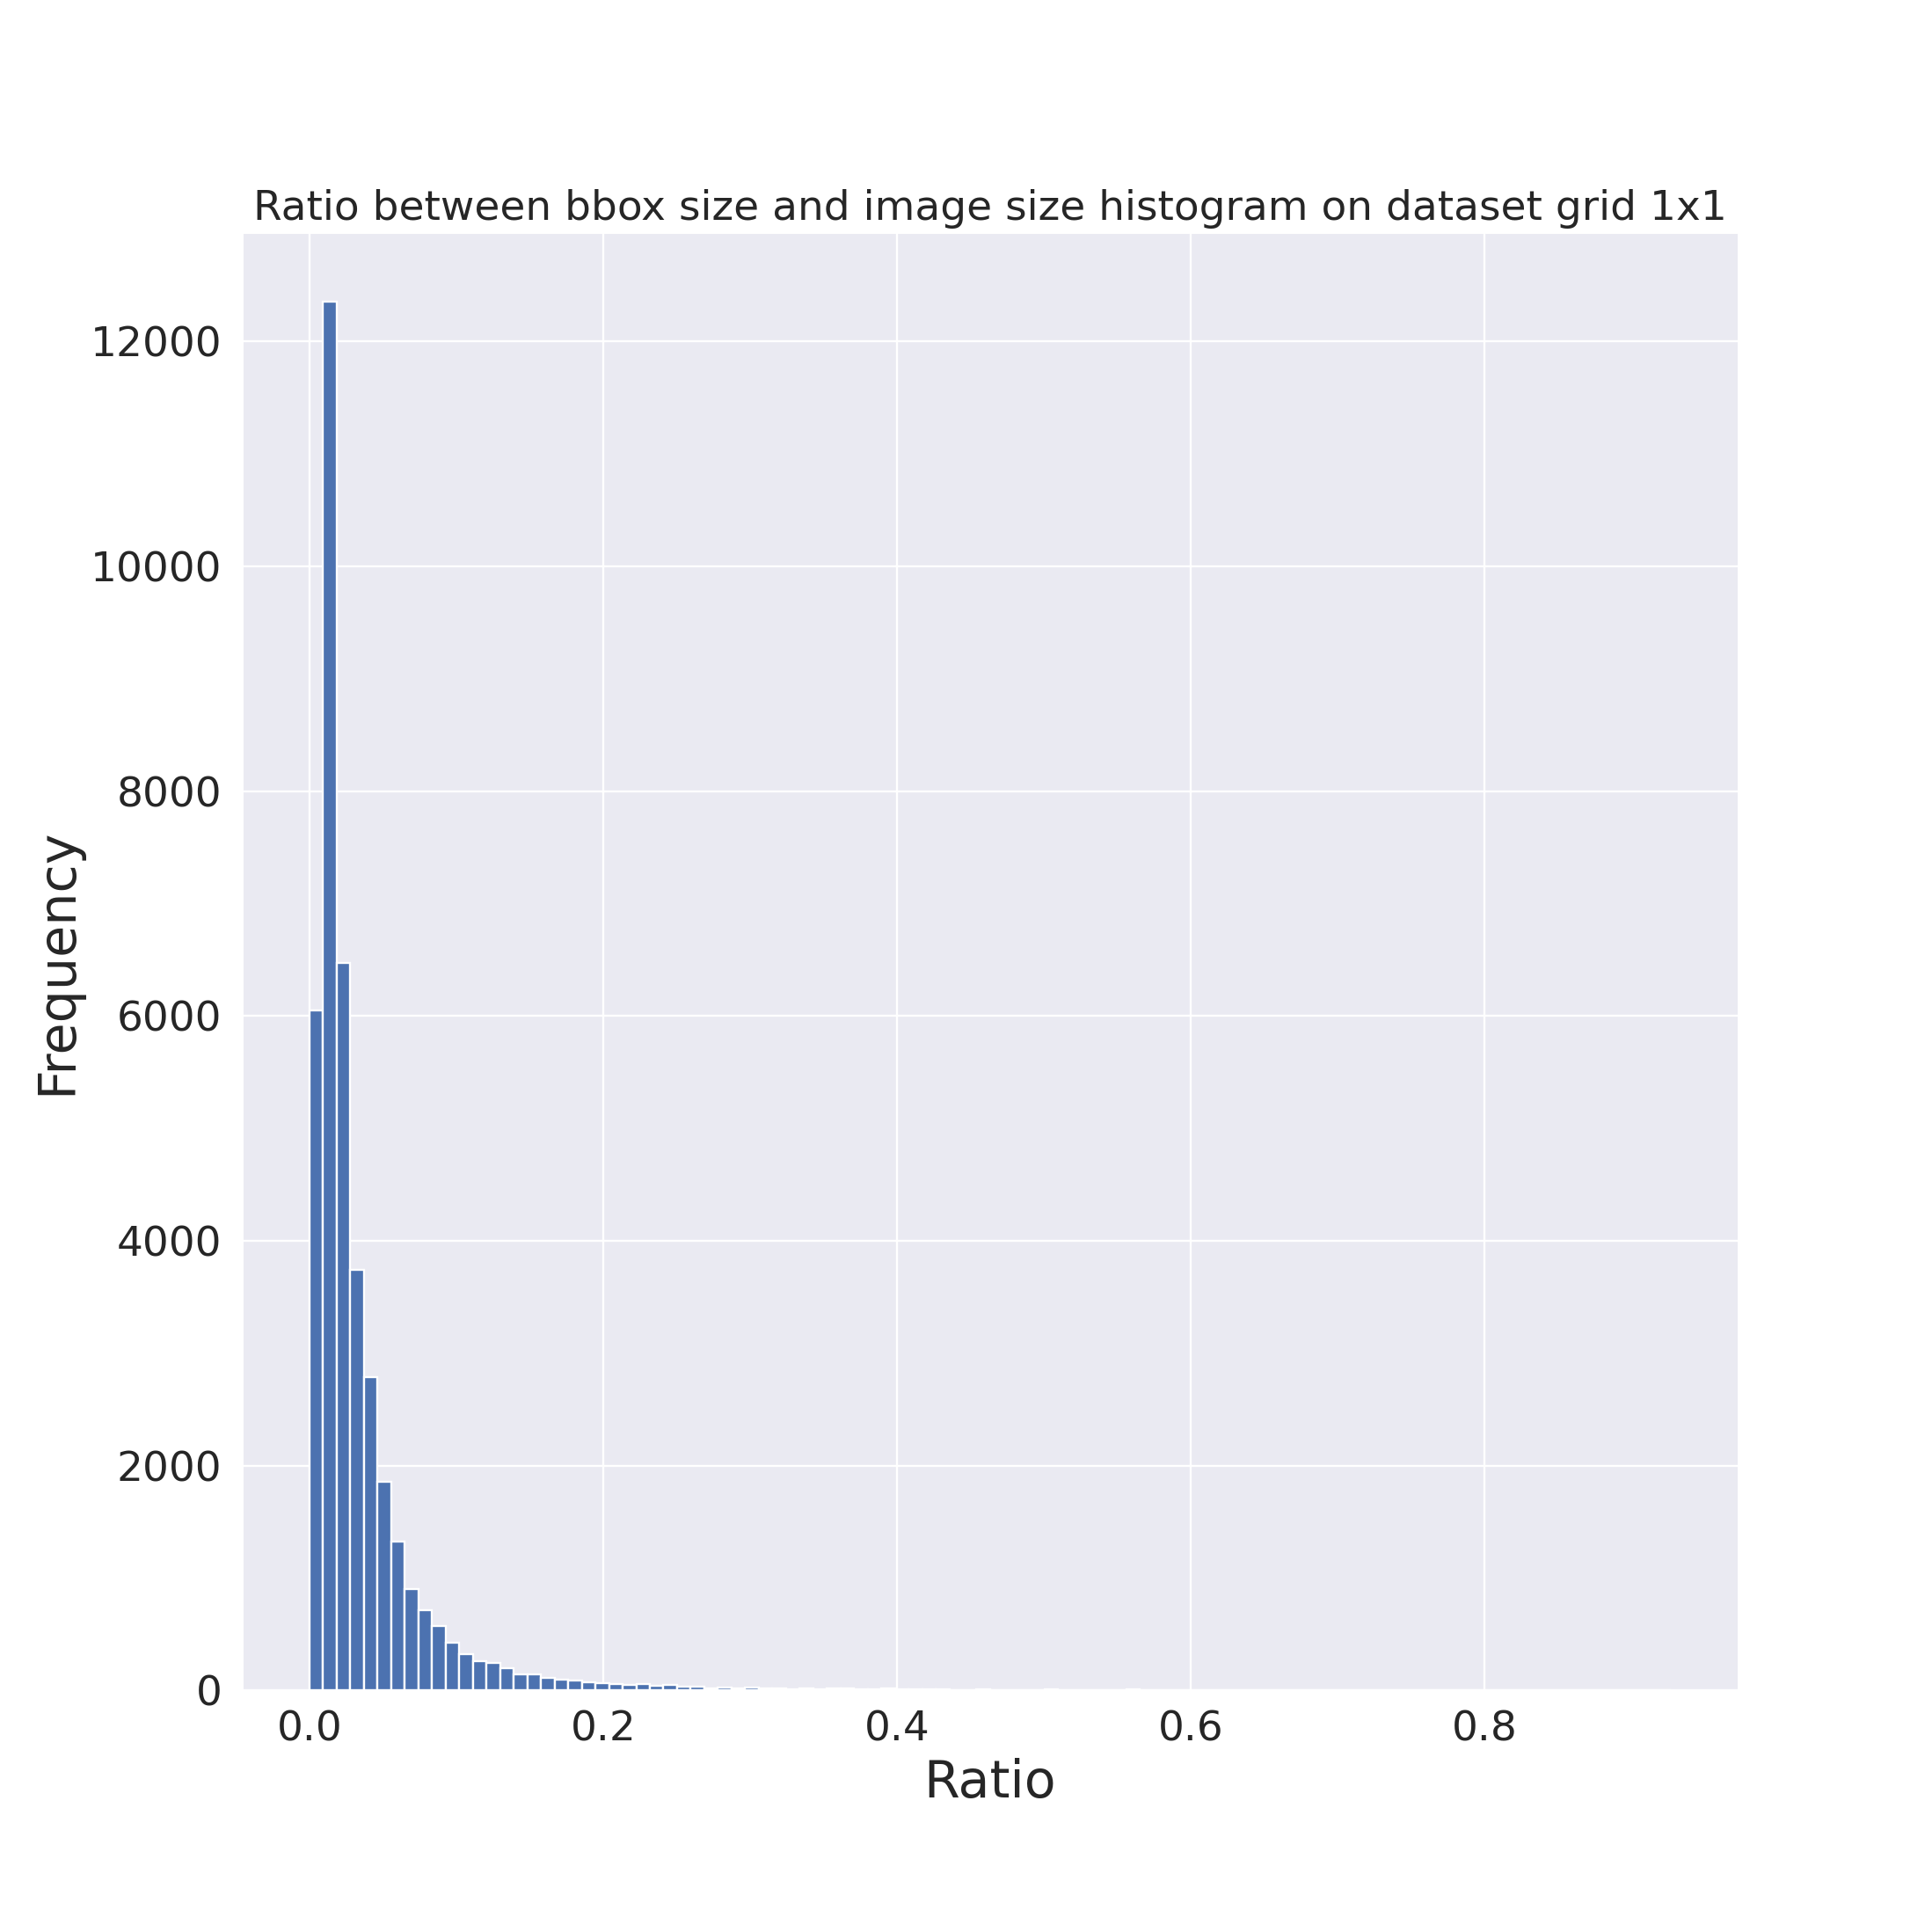
\includegraphics[width=5.3cm]{images/widerface_nk_scale_1K}}
        \subfigure[]{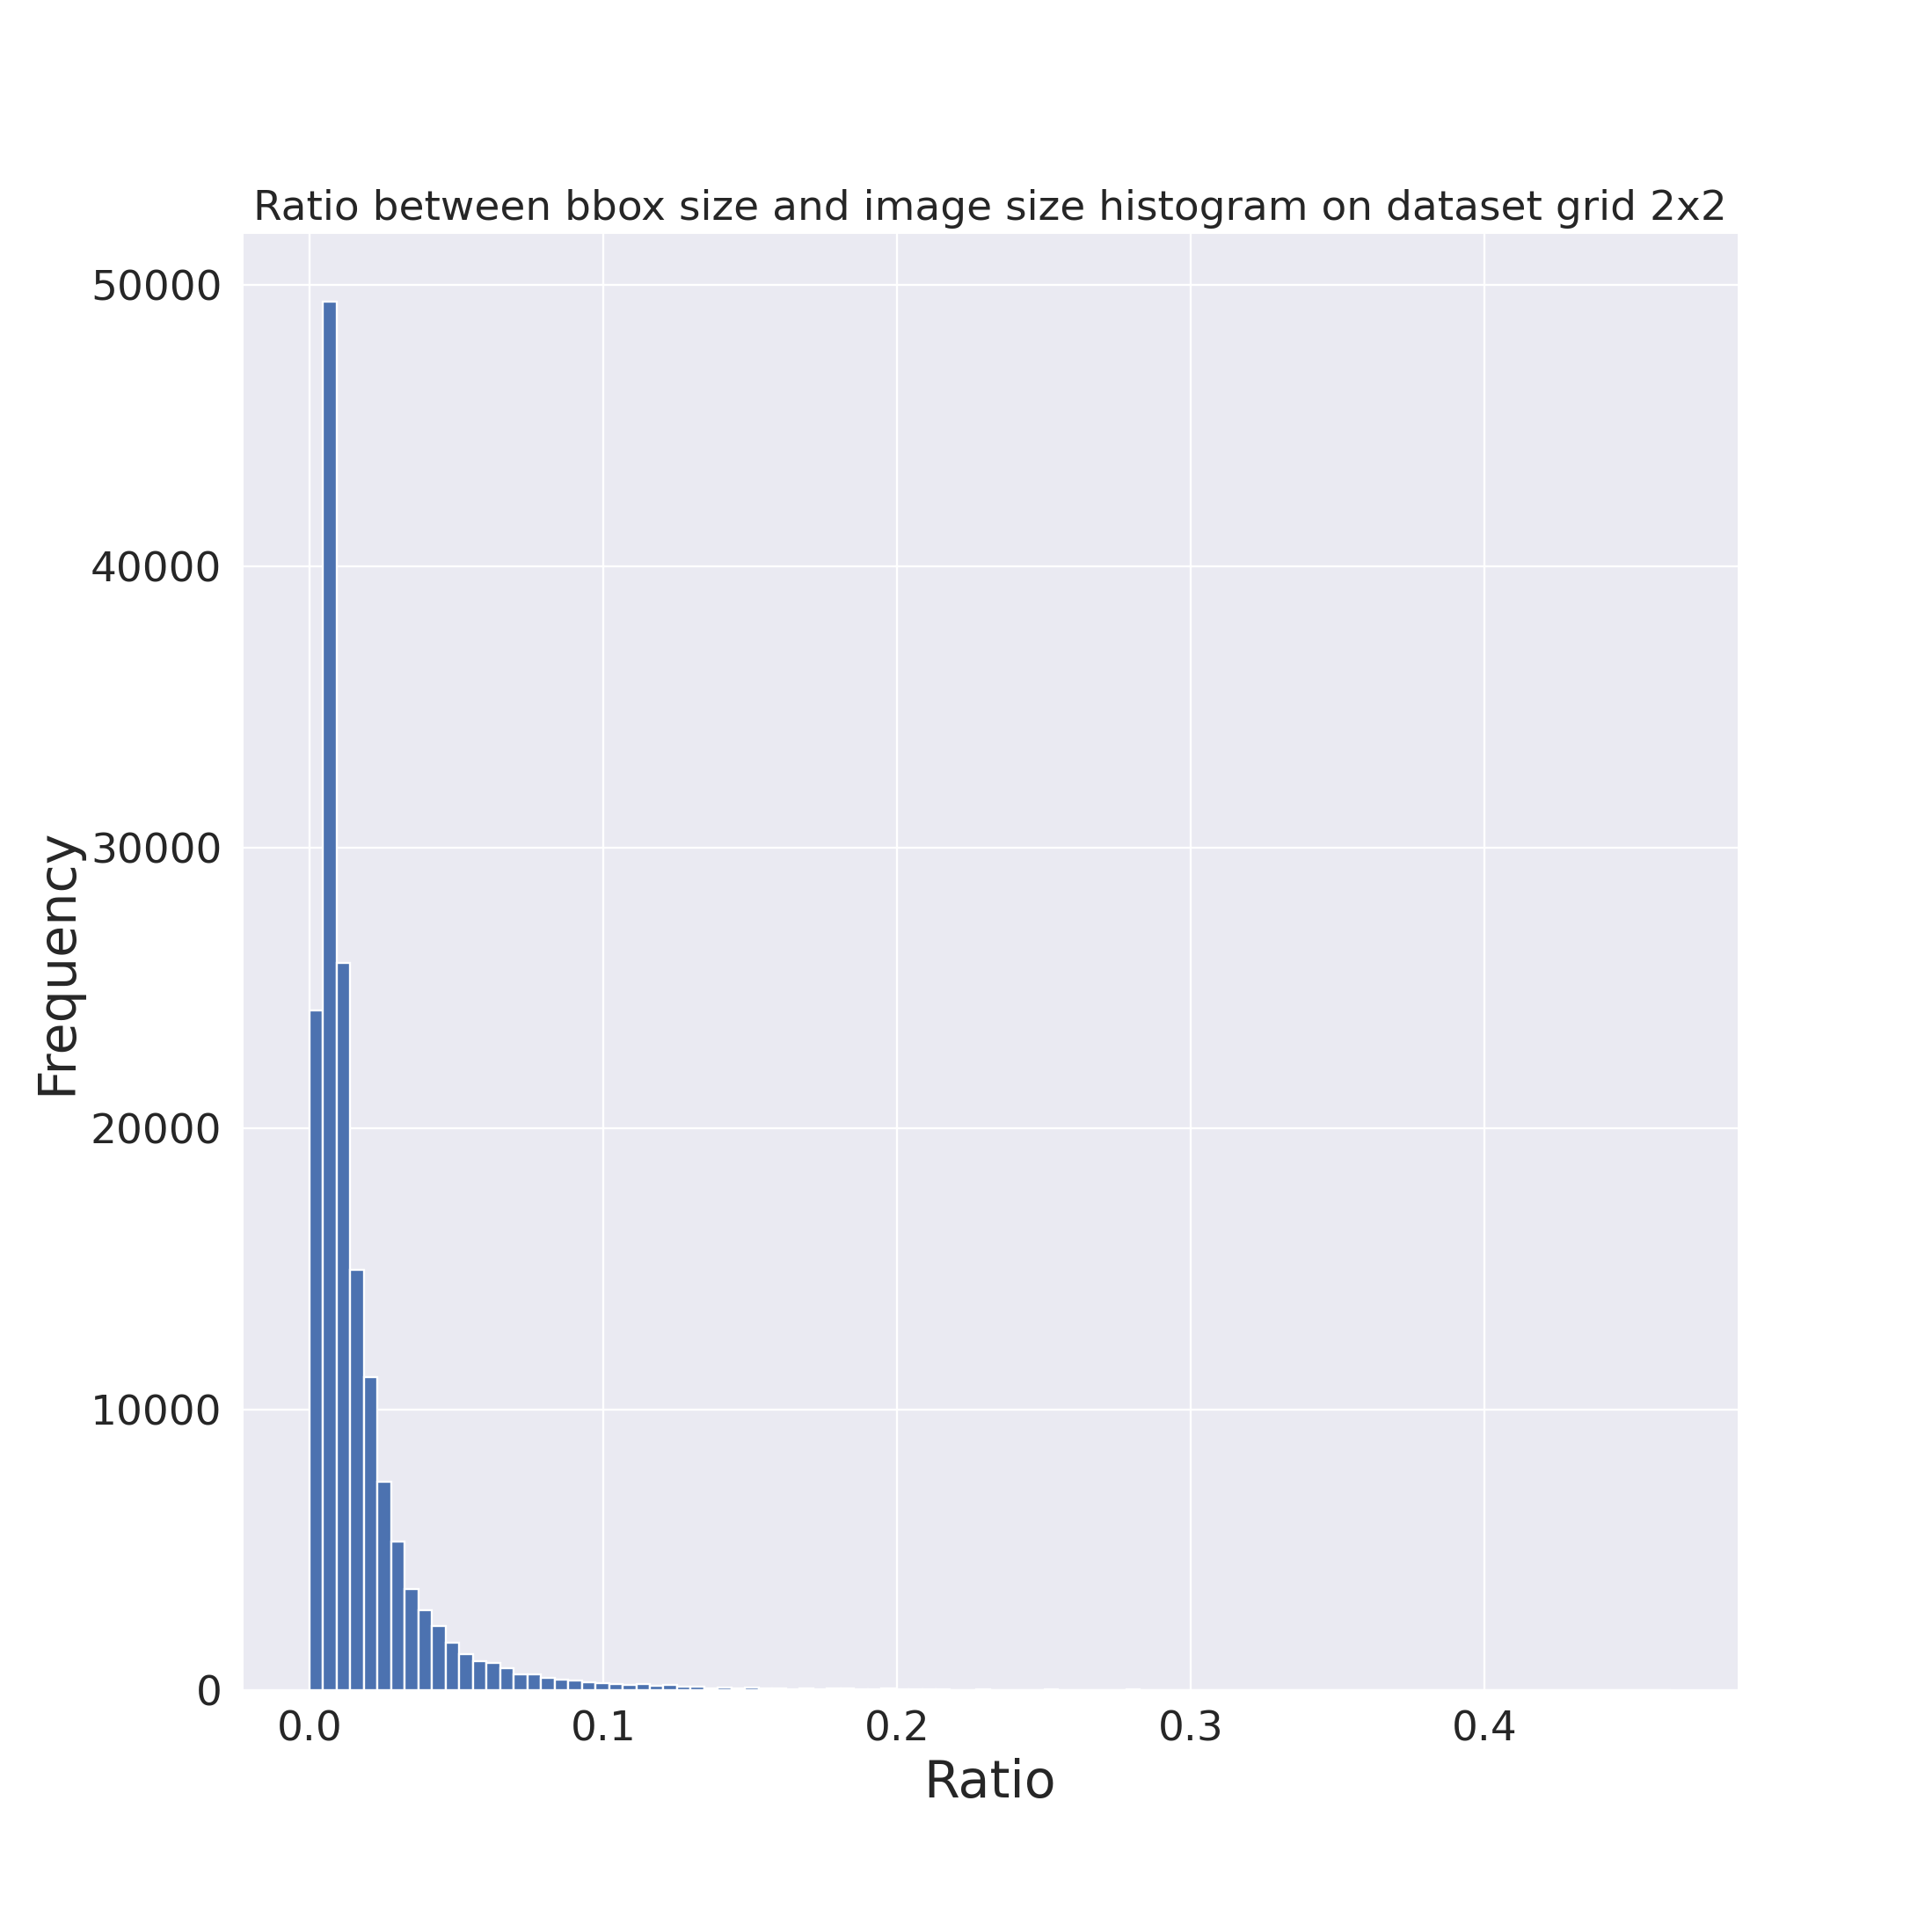
\includegraphics[width=5.3cm]{images/widerface_nk_scale_2K}}
        \subfigure[]{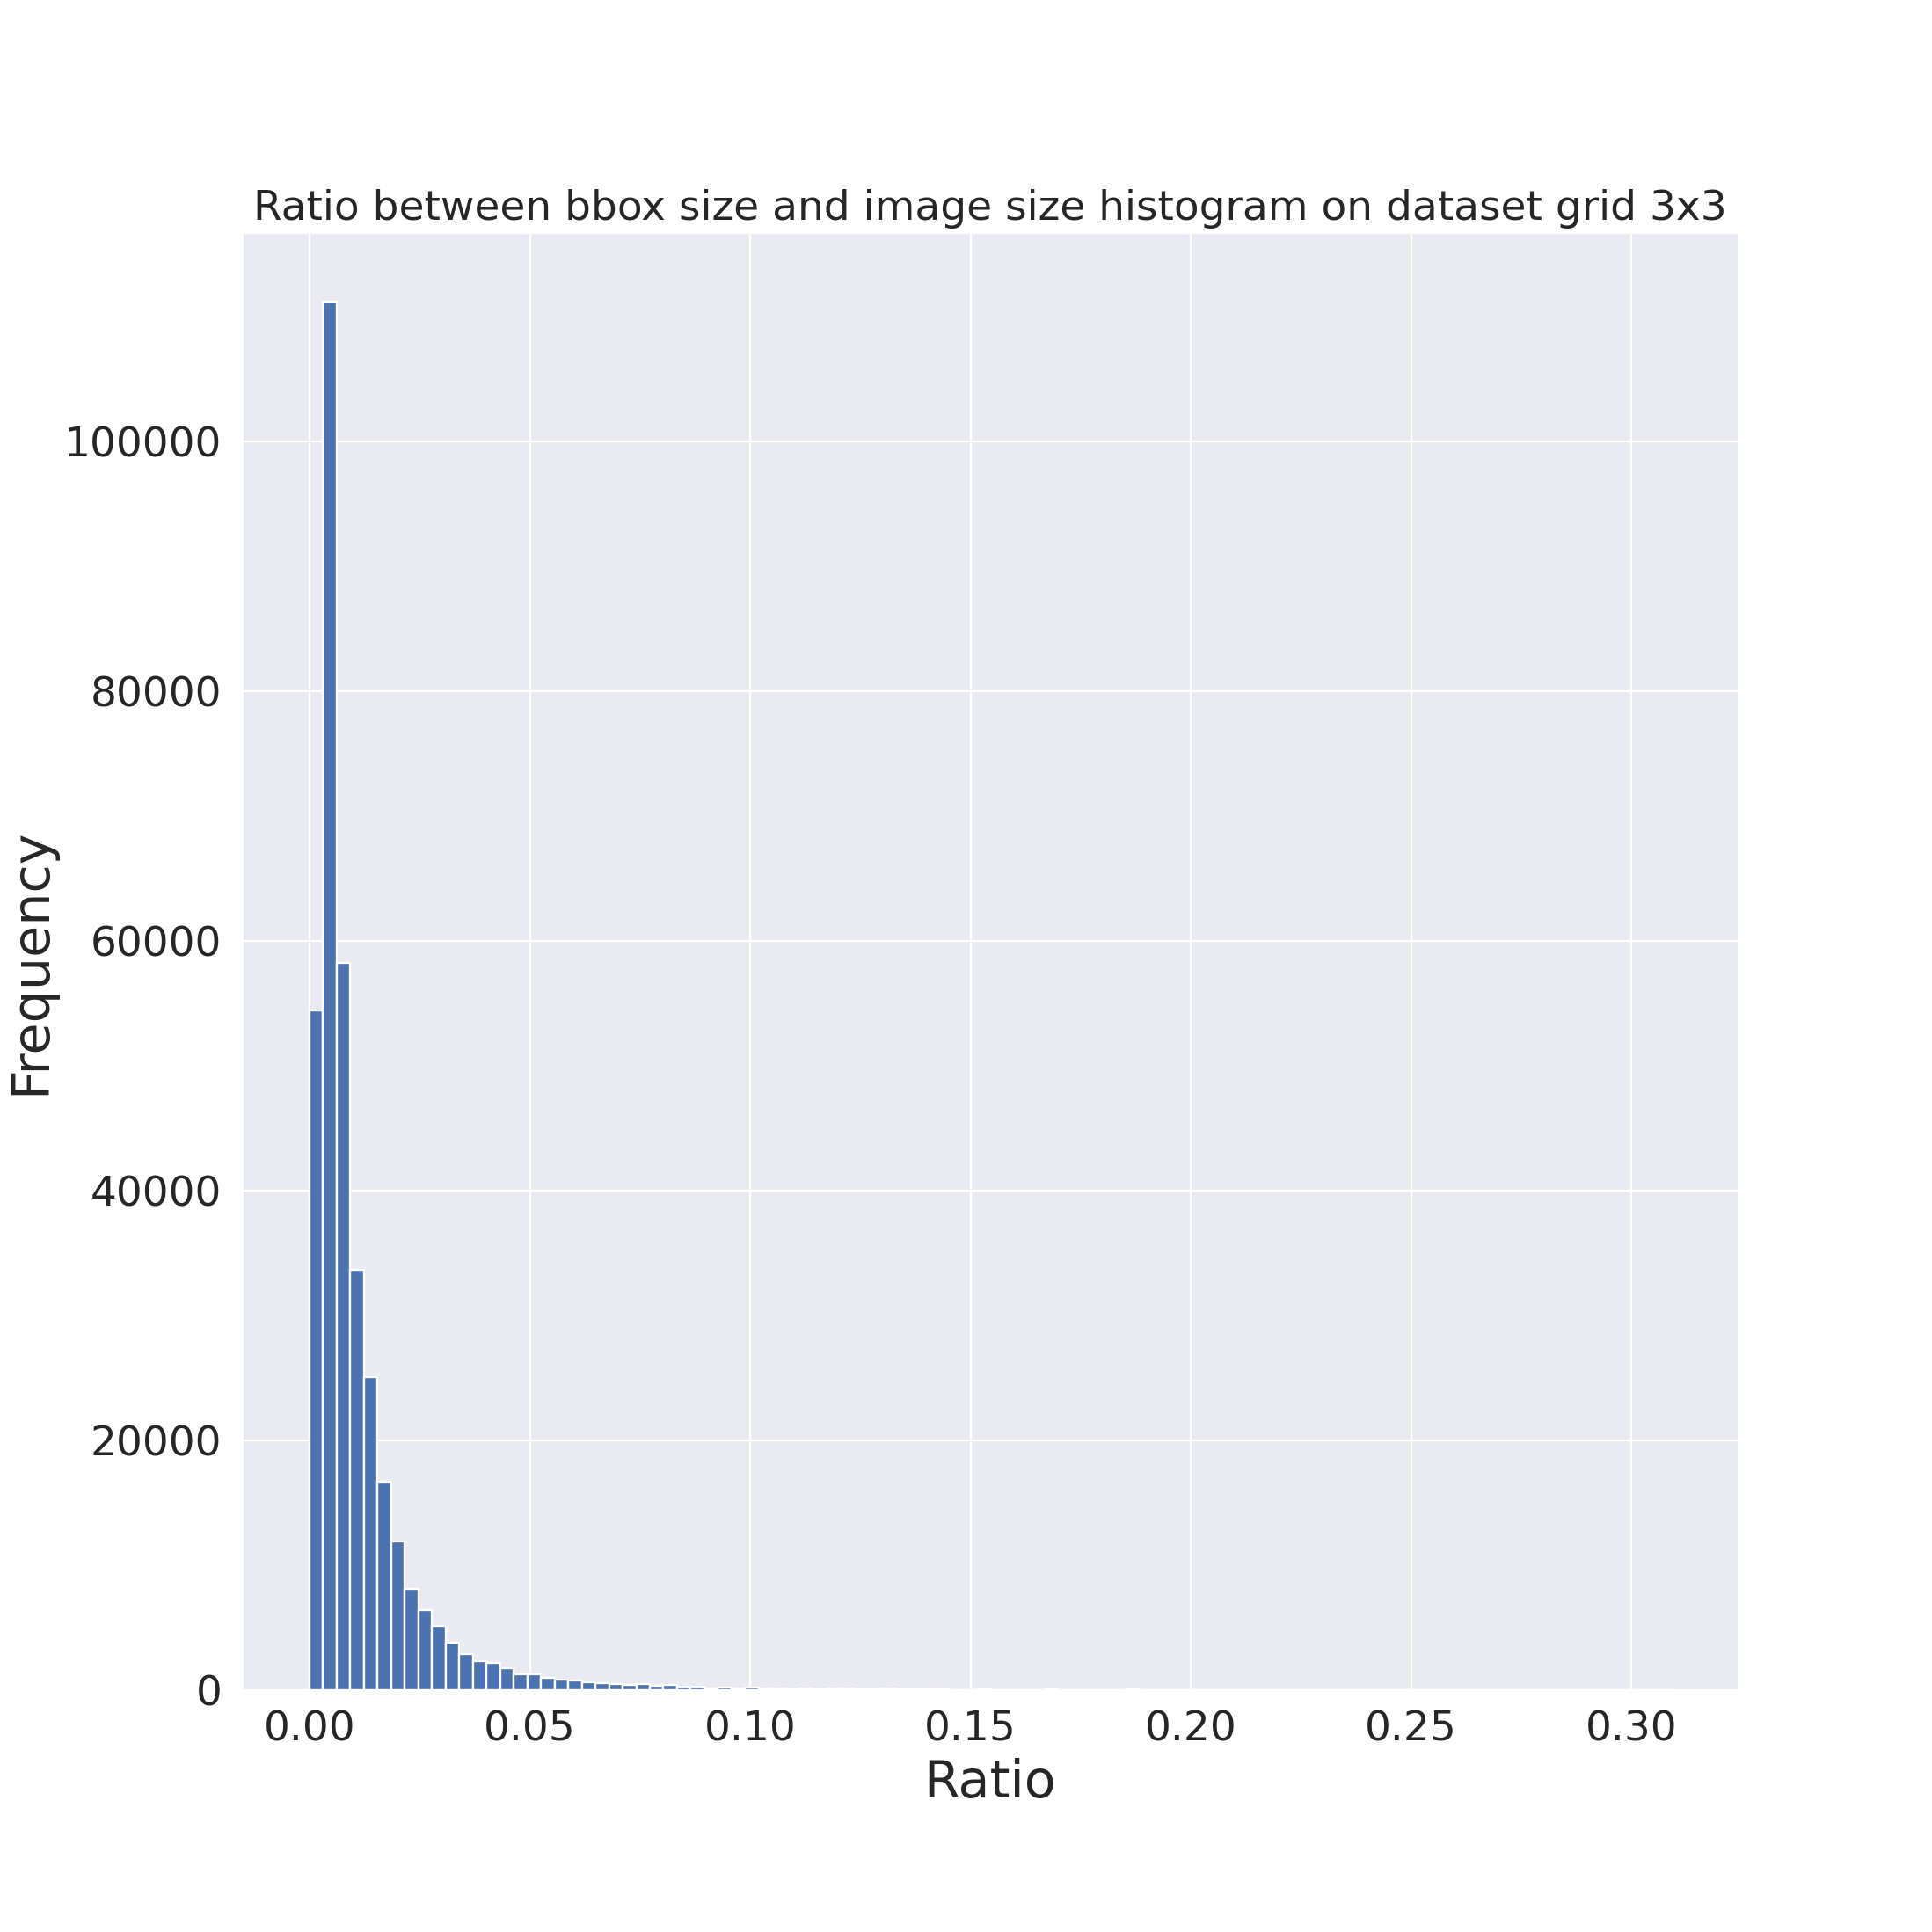
\includegraphics[width=5.3cm]{images/widerface_nk_scale_3K}}
        \subfigure[]{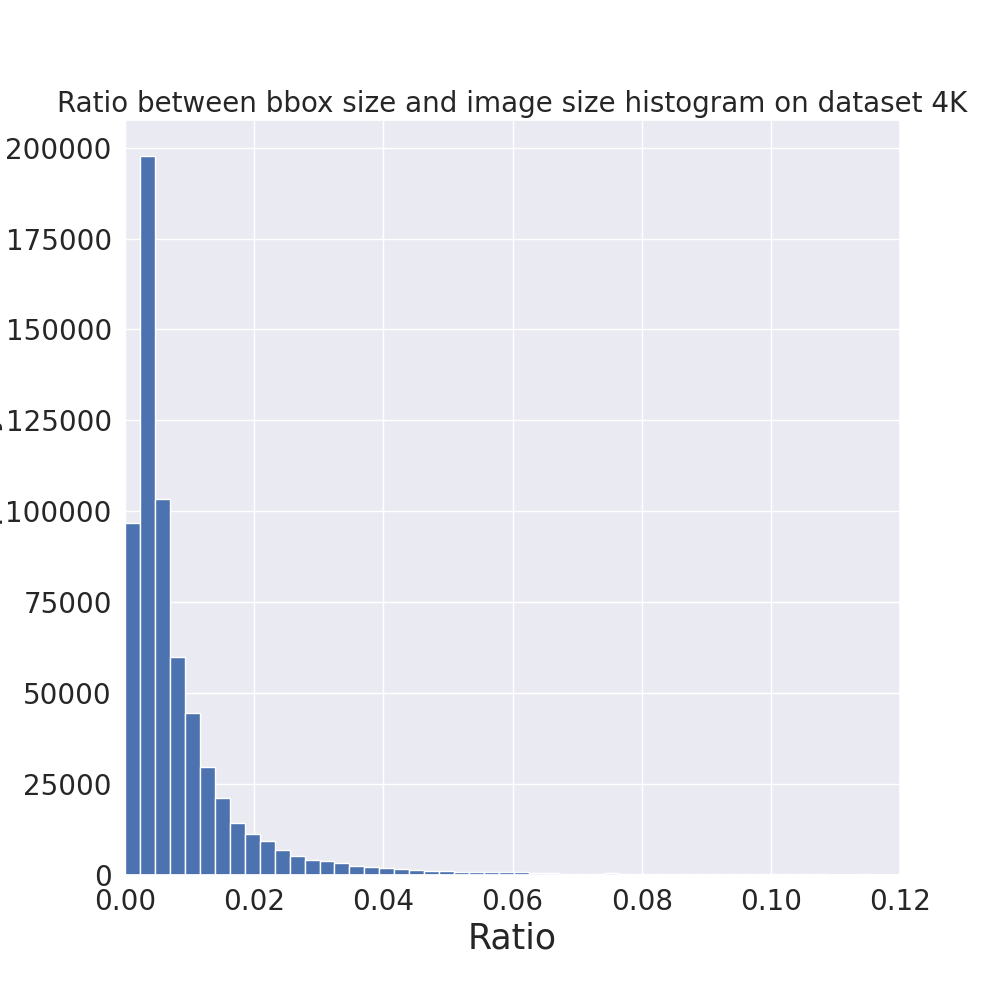
\includegraphics[width=5.3cm]{images/widerface_nk_scale_4K}}
        \subfigure[]{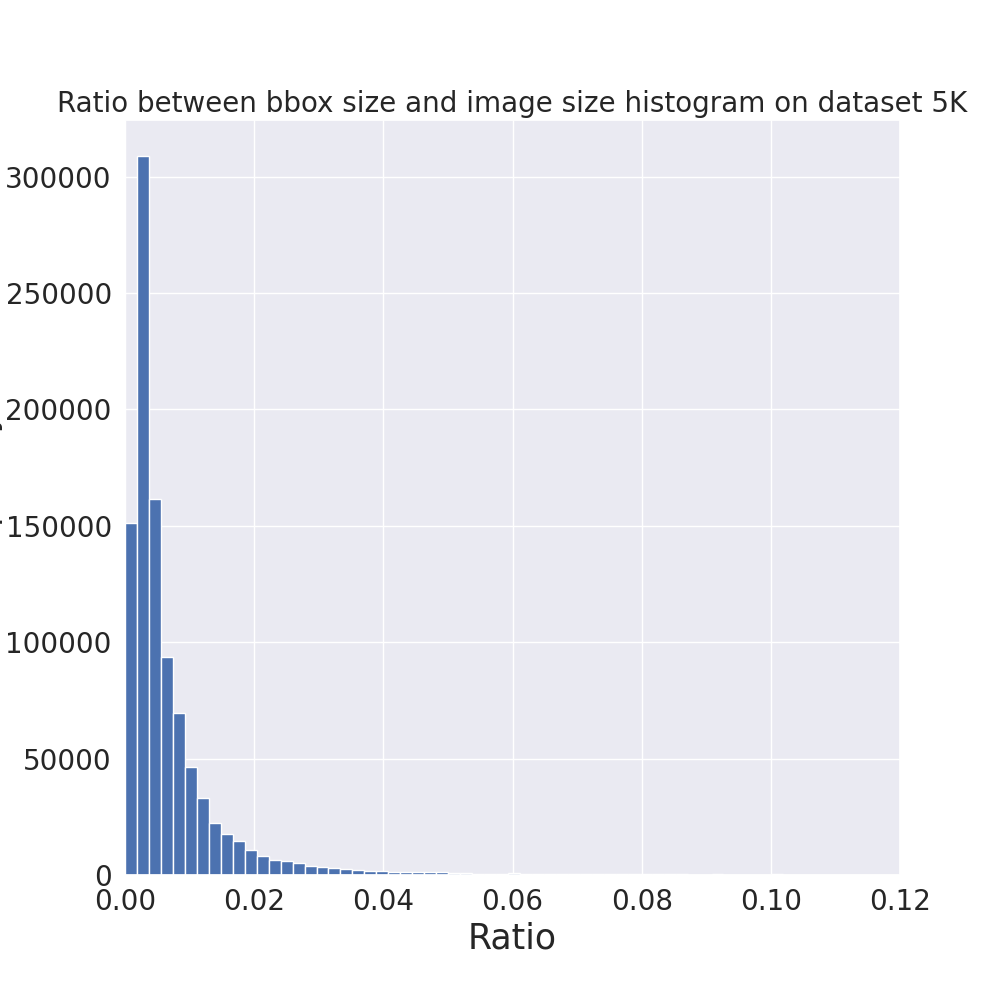
\includegraphics[width=5.3cm]{images/widerface_nk_scale_5K}}
        \caption{Phân phối về tỷ lệ giữa kích thước của hộp giới hạn và kích thước ảnh trong bộ dữ liệu WIDER FACE \cite{yang2016wider} (a) so sánh với bộ dữ liệu WIDER FACE 4K dạng lưới $2 \times 2$ (b), $3 \times 3$ (c), $4 \times 4$ (d) và $5 \times 5$ (d)}
        \label{fig:widerface_4k_scale}
    \end{figure}

    \noindent
    Đối với bộ dữ liệu WIDER FACE 4K, trung bình kích thước hộp giới hạn của khuôn mặt bằng khoảng 1\% kích thước của ảnh đối với dạng lưới $2 \times 2$, 0.6\% kích thước của ảnh đối với dạng lưới $3 \times 3$, 0.5\% kích thước của ảnh đối với dạng lưới $4 \times 4$ và 0.3\% kích thước của ảnh đối với dạng lưới $5 \times 5$.

    \noindent
    Với những thông số trên, bộ dữ liệu WIDER FACE 4K được kỳ vọng giúp đánh giá khách quan độ chính xác và tốc độ của các mô hình giải bài toán nhận diện khuôn mặt với ảnh chất lượng cao.
}